\documentclass[reprint,  amsmath,  amssymb,  pra,  nofootinbib,  a4paper]{revtex4-2}
\usepackage{xeCJK}
\usepackage{graphicx}
\usepackage{gensymb}
\usepackage{multirow,  dcolumn}
\usepackage{bm,  physics}
\usepackage{url}
\usepackage[load=addn]{siunitx}
\usepackage{float}
\usepackage{braket}
\usepackage{pst-optexp}
\usepackage{tipa}
\makeatletter
\newcommand{\cemph}[1]{\@tfor\i:=#1\do{\textsubdot{\textit{\i}}}}
\makeatother
\usepackage[labelformat=simple]{subcaption}
\usepackage[justification=raggedright]{caption}
\renewcommand\thesubfigure{(\alph{subfigure})}
\definecolor{link}{RGB}{46, 48, 146}
%\usepackage{subfigure}
\usepackage[explicit, indentafter]{titlesec}
\titlespacing*{\section}{2pt}{9pt}{9pt}
\newcommand{\perc}[1]{\SI{#1}{\percent}}
\newcommand{\csAtom}{${}^{137}\text{Cs}$}
\newcommand{\coAtom}{${}^{60}\text{Co}$}
\usepackage{setspace}
\setlength{\parindent}{2em}
\setlength{\parskip}{0.3em}
\linespread{1.4}

\usepackage{caption}
\captionsetup[figure]{labelfont={bf}, name={图}}
\captionsetup[table]{labelfont={bf}, name={表}}
\captionsetup{font={small}}

\usepackage{hyperref}
\hypersetup{
    % bookmarksnumbered, 
    breaklinks, 
    colorlinks, 
    citecolor=link, 
    urlcolor=link, 
    linkcolor=link
}
\usepackage{bookmark}
% \bookmarksetup{startatroot}

\begin{document}

\title{康普顿效应验证实验}
%\thanks{本文为2018级本科生顾周洲(学号\href{mailto:zzgu@pku.edu.cn}{1800011320})和陈天扬(学号\href{mailto:chentianyang@pku.edu.cn}{1800011327})在2019-2020学年进行的研究性实验工作的总结报告,作者按学号排序、不分先后.指导教师为张朝晖老师和王伟老师.}

\author{顾周洲}
%\email[邮箱:]{zhangzh@pku.edu.cn}
\affiliation{北京大学物理学院\\ 中国,北京,颐和园路5号\ 100871}
\collaboration{2021年 10 月}

\begin{abstract}
    本实验以\csAtom 为放射源,测定了其放射出的\SI{0.662}{MeV} $\gamma$射线被铝棒散射后的能量及相对微分散射截面关于散射角的分布。实验结果与康普顿散射的光子能量随散射角、以及Klein–Nishina 公式给出的散射截面随散射角变化关系符合得相当好,进一步分析对实验的误差给出了解释,从而验证了对康普顿效应的理论计算。


\end{abstract}

\maketitle
%\tableofcontents

\section{引言}

\section{理论}
	\begin{equation}
        f=ma
    \end{equation}
\section{实验}
\subsection{实验装置}

\begin{figure*}[tbp]
        \centering
         \vskip\baselineskip
        \begin{subfigure}[b]{0.45\textwidth}
            \centering
            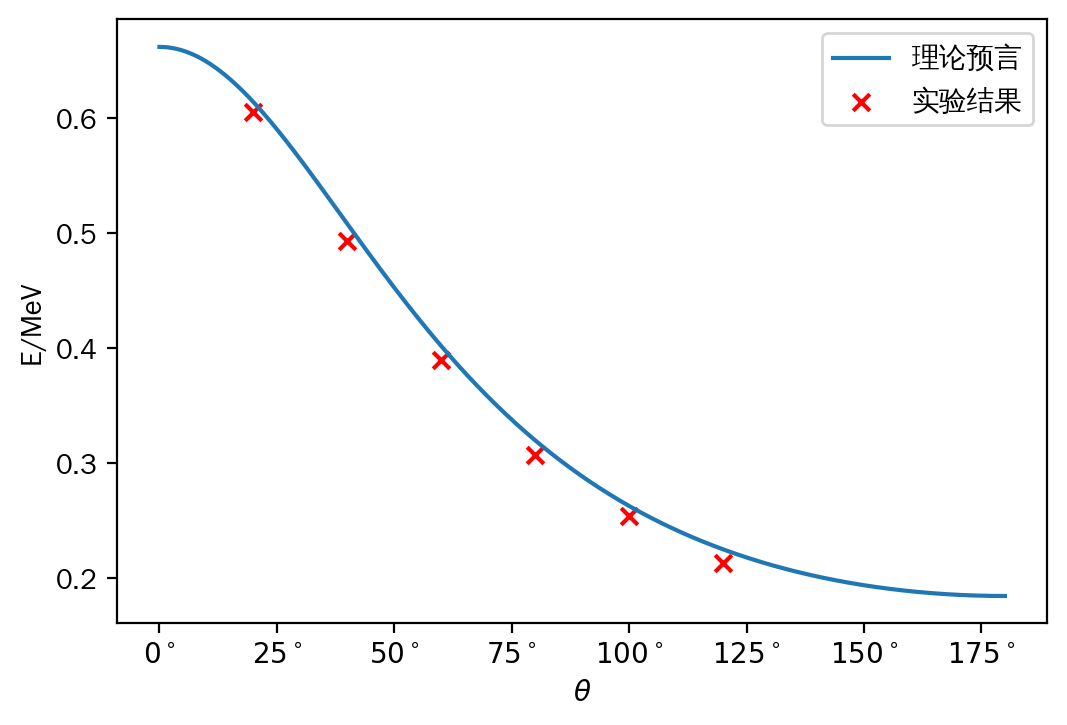
\includegraphics[width=\textwidth]{pic/energy.png}
            \caption{}
            \label{fig:single}
        \end{subfigure}
        \hfill
       \begin{subfigure}[b]{0.45\textwidth}
            \centering
            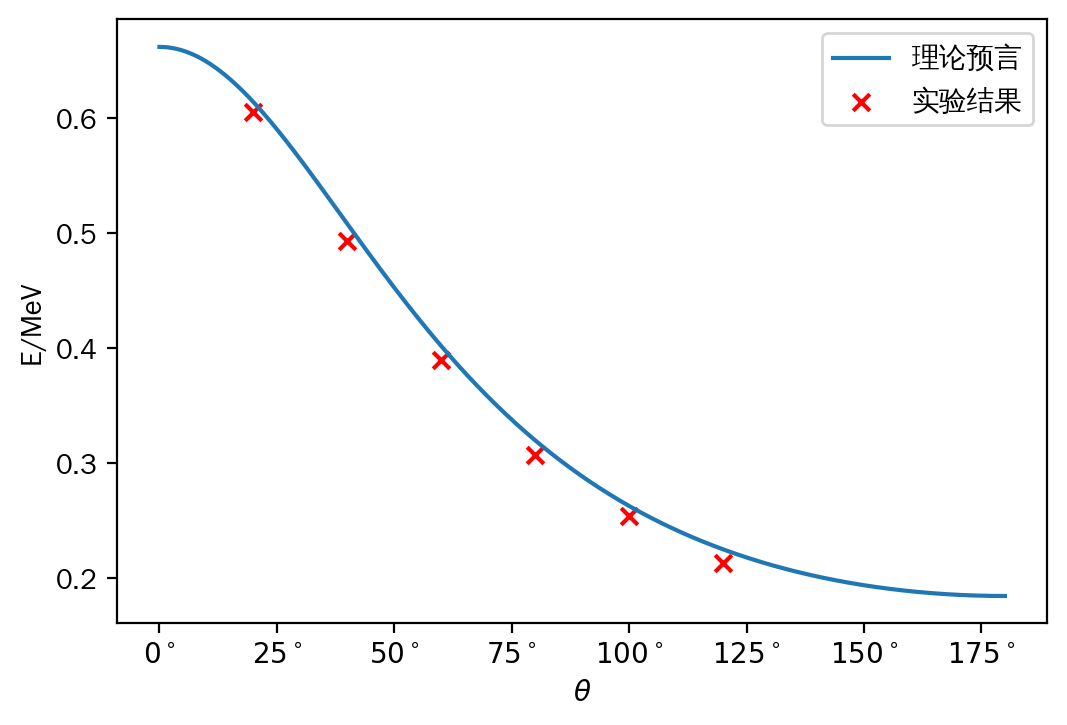
\includegraphics[width=\textwidth]{pic/energy.png}
            \caption{}
            \label{fig:multi}
        \end{subfigure}
        \caption{xxxx}
        \label{fig:exp_channel}
    \end{figure*}

\section{结论}
本实验以 \csAtom 为放射源,考察了 ${662}\text{keV}$ 光子散射后的能量角分布及相对微分散射截面角分布,结果与康普顿等人的理论预计基本一致,可以说是验证了康普顿效应。	实验简要分析了可能的误差来源,计算了有限立体角效应对于实验结果的影响,强调了周围墙体散射可能带来的显著影响;建议更为精确的测定应当在尽可能减小二次散射的空旷环境中进行。
\begin{acknowledgments}
感谢老师对实验的细致讲解, 以xxxxx促进我对xxxxx更深理解.

\end{acknowledgments}
\appendix
\section{思考题思考题思考题}

\begin{thebibliography}{99}
    \bibitem{taylor2004modern} TAYLOR J R, DUBSON M A, ZAFIRATOS C D. Modern physics for scientists and engineers[M]. [S.l.]: Prentice-Hall, 2004.
    \bibitem{compton1923quantum} COMPTON A H. A quantum theory of the scattering of x-rays by light elements[J]. Physical review, 1923, 21(5): 483.
    \bibitem{textbook}吴思诚, 荀坤, 近代物理实验 第四版 (高等教育出版社,2015).
    \bibitem{woo1926distribution} WOO Y. The distribution of energy between the modified and the unmodified rays in the compton effect[J]. physical Review, 1926, 27(2): 119.
    \end{thebibliography}
\end{document}
